% imports
\documentclass[11pt, reqno]{amsart}
\usepackage[margin=1in]{geometry} 
\usepackage{multicol}

% \geometry{letterpaper}       
%\geometry{landscape}                % Activate for for rotated page geometry
\usepackage[parfill]{parskip}    % Deactivate to begin paragraphs with an indent rather than an empty line
\setlength{\parindent}{20pt}   
\usepackage{amsfonts, amscd, amssymb, amsthm, amsmath}
\usepackage{pdfsync}  %leaves makers for tex searching
\usepackage{enumerate}
\usepackage{enumitem}
\usepackage{multicol}
\usepackage[pdftex,bookmarks]{hyperref}
\usepackage{biblatex}
\usepackage{graphicx}				   % For importing photos. 
\usepackage{caption}           % centering captions
\usepackage{float}
\setcounter{tocdepth}{3}
\setcounter{secnumdepth}{3}
\let\oldtocsection=\tocsection

\let\oldtocsubsection=\tocsubsection

\let\oldtocsubsubsection=\tocsubsubsection

\DeclareFieldFormat{postnote}{#1}

\renewcommand{\tocsection}[2]{\hspace{0em}\oldtocsection{#1}{#2}}
\renewcommand{\tocsubsection}[2]{\hspace{1em}\oldtocsubsection{#1}{#2}}
\renewcommand{\tocsubsubsection}[2]{\hspace{2em}\oldtocsubsubsection{#1}{#2}}

\addbibresource{bib.bib} % Import the bibliography
\graphicspath{ {./images/} }


\hypersetup{
  colorlinks=true,
  allcolors=blue
}

%%% Theorems %%%--------------------------------------------------------- 
\theoremstyle{plain}
    \newtheorem{thm}{Theorem}[section]
    \numberwithin{thm}{subsection}
    \newtheorem{lemma}[thm]{Lemma}
    \newtheorem{prop}[thm]{Proposition}
    \newtheorem{cor}[thm]{Corollary}
    \newtheorem{fact}[thm]{Fact}
\theoremstyle{definition}
    \newtheorem{defn}[thm]{Definition}
    \newtheorem{remark}{Remark}


%%% Environments %%%--------------------------------------------------------- 
\newenvironment{ans}{\color{black}\medskip \paragraph*{\emph{Answer}.}}{\hfill \break  $~\!\!$ \dotfill \medskip }
\newenvironment{sketch}{\medskip \paragraph*{\emph{Proof sketch}.}}{ \medskip }
\newenvironment{summary}{\medskip \paragraph*{\emph{Summary}.}}{  \hfill \break  \rule{1.5cm}{0.4pt} \medskip }
\newcommand\Ans[1]{\color{black}\hfill \emph{Answer:} {#1}}


%%% Pictures %%%--------------------------------------------------------- 
%%% If you need to draw pictures, tikzpicture is one good option. Here are some basic things I always use:
\usepackage{tikz}
\usetikzlibrary{arrows, decorations.text,calc,arrows.meta}
\tikzstyle{V}=[draw, fill =black, circle, inner sep=0pt, minimum size=2pt]
\tikzstyle{bV}=[draw, fill =black, circle, inner sep=0pt, minimum size=3.5pt]
\newcommand\TikZ[1]{\begin{matrix}\begin{tikzpicture}#1\end{tikzpicture}\end{matrix}}
\definecolor{r}{RGB}{227, 242, 253}
\definecolor{o}{RGB}{187, 222, 251}
\definecolor{y}{RGB}{144, 202, 249}
\definecolor{g}{RGB}{66, 165, 245}
\definecolor{b}{RGB}{30, 136, 229}

%%% Color  %%%---------------------------------------------------------
\usepackage{color}
\newcommand{\blue}[1]{{\color{blue}#1}}
\newcommand{\NOTE}[1]{{\color{blue}#1}}
\newcommand{\MOVED}[1]{{\color{gray}#1}}


%%% Alphabets %%%---------------------------------------------------------
%%% Some shortcuts for my commonly used special alphabets and characters.
\def\cA{\mathcal{A}}\def\cB{\mathcal{B}}\def\cC{\mathcal{C}}\def\cD{\mathcal{D}}\def\cE{\mathcal{E}}\def\cF{\mathcal{F}}\def\cG{\mathcal{G}}\def\cH{\mathcal{H}}\def\cI{\mathcal{I}}\def\cJ{\mathcal{J}}\def\cK{\mathcal{K}}\def\cL{\mathcal{L}}\def\cM{\mathcal{M}}\def\cN{\mathcal{N}}\def\cO{\mathcal{O}}\def\cP{\mathcal{P}}\def\cQ{\mathcal{Q}}\def\cR{\mathcal{R}}\def\cS{\mathcal{S}}\def\cT{\mathcal{T}}\def\cU{\mathcal{U}}\def\cV{\mathcal{V}}\def\cW{\mathcal{W}}\def\cX{\mathcal{X}}\def\cY{\mathcal{Y}}\def\cZ{\mathcal{Z}}

\def\AA{\mathbb{A}} \def\BB{\mathbb{B}} \def\CC{\mathbb{C}} \def\DD{\mathbb{D}} \def\EE{\mathbb{E}} \def\FF{\mathbb{F}} \def\GG{\mathbb{G}} \def\HH{\mathbb{H}} \def\II{\mathbb{I}} \def\JJ{\mathbb{J}} \def\KK{\mathbb{K}} \def\LL{\mathbb{L}} \def\MM{\mathbb{M}} \def\NN{\mathbb{N}} \def\OO{\mathbb{O}} \def\PP{\mathbb{P}} \def\QQ{\mathbb{Q}} \def\RR{\mathbb{R}} \def\SS{\mathbb{S}} \def\TT{\mathbb{T}} \def\UU{\mathbb{U}} \def\VV{\mathbb{V}} \def\WW{\mathbb{W}} \def\XX{\mathbb{X}} \def\YY{\mathbb{Y}} \def\ZZ{\mathbb{Z}}  

\def\fa{\mathfrak{a}} \def\fb{\mathfrak{b}} \def\fc{\mathfrak{c}} \def\fd{\mathfrak{d}} \def\fe{\mathfrak{e}} \def\ff{\mathfrak{f}} \def\fg{\mathfrak{g}} \def\fh{\mathfrak{h}} \def\fj{\mathfrak{j}} \def\fk{\mathfrak{k}} \def\fl{\mathfrak{l}} \def\fm{\mathfrak{m}} \def\fn{\mathfrak{n}} \def\fo{\mathfrak{o}} \def\fp{\mathfrak{p}} \def\fq{\mathfrak{q}} \def\fr{\mathfrak{r}} \def\fs{\mathfrak{s}} \def\ft{\mathfrak{t}} \def\fu{\mathfrak{u}} \def\fv{\mathfrak{v}} \def\fw{\mathfrak{w}} \def\fx{\mathfrak{x}} \def\fy{\mathfrak{y}} \def\fz{\mathfrak{z}}
\def\fgl{\mathfrak{gl}}  \def\fsl{\mathfrak{sl}}  \def\fso{\mathfrak{so}}  \def\fsp{\mathfrak{sp}}  
\def\GL{\mathrm{GL}} \def\SL{\mathrm{SL}}  \def\SP{\mathrm{SP}} \def\O{\mathrm{O}}

\def\<{\langle} \def\>{\rangle}
\usepackage{mathabx}
\def\acts{\lefttorightarrow}
\def\ad{\mathrm{ad}} 
\def\Aut{\mathrm{Aut}}
\def\Ann{\mathrm{Ann}}
\def\dim{\mathrm{dim}} 
\def\End{\mathrm{End}} 
\def\ev{\mathrm{ev}} 
\def\Fr{\mathcal{F}\mathrm{r}}
\def\half{\hbox{$\frac12$}}
\def\Hom{\mathrm{Hom}} 
\def\id{\mathrm{id}} 
\def\sgn{\mathrm{sgn}}  
\def\supp{\mathrm{supp}}  
\def\Tor{\mathrm{Tor}}
\def\tr{\mathrm{tr}} 
\def\vep{\varepsilon}
\def\f{\varphi}
\def\im{\mathrm{im}}
\def\st{\;|\;}
\def\ses{0\rightarrow X \xrightarrow{f} Y \xrightarrow{g} Z \rightarrow 0}


\def\Obj{\mathrm{Obj}}
\def\normeq{\unlhd}
\def\Set{{\cS\mathrm{et}}}
\def\Fin{{\cF\mathrm{inSet}}}
\def\Set{{\cS\mathrm{et}}}
\def\Grp{{\cG\mathrm{rp}}}
\def\Ab{{\cA\mathrm{b}}}
\def\Mod{{\cM\mathrm{od}}}
\def\ab{\mathrm{ab}}
\def\lcm{\mathrm{lcm}}
\def\ZZn{\ZZ/n\ZZ}
\def\CS3{\CC S_3}



\newcommand{\Hint}[1]{\hfill{\small [\emph{Hint:} {#1}]}}
\newcommand\Cmd[1]{$\backslash$\texttt{#1}}
\newcommand{\SES}[5]{0 \hookrightarrow {#1} \xrightarrow{{#4}} {#2} \xrightarrow{{#5}} {#3} \rightarrow 0}

%%%%%%%%%%%%%%%%%%%%%%%%%%%%%% 
%%%%%%%%%%%%%%%%%%%%%%%%%%%%%%

\title{Course Summary}
\author{Gabriela Brown\\ Symbolic Dynamics - Wolf \\ Spring 2023}

\begin{document}
\maketitle

 {
  \setlength{\parskip}{4.4pt}   
  \tableofcontents
 }


\section{Introduction}
% TODO

\section{Fundamentals of Shift Spaces}
\cite{lind-marc}[C.1,C.2]

% Key realizations: 
% \begin{itemize}
% \item The topology (open sets) of a shift space has a basis in cylinder sets. It is thus natural to define a shift space by forbidden words, because we need the shift space to be closed, and the forbidden words give us a countable number open sets that are excluded, the union of which is open, and the complement of which is closed.

% \item Why do we bother with progressive overlap? (i.e. using Nth higher block shift vs Nth higher power shift) Both are shift spaces, but the former are what give us ``sliding block codes" (through factoring?) which when they are invertible are what give us topological conjugacies between shift spaces. Higher block shifts come up later in the Finite Coding Theorem to get around a particular entropy requirement. 

% \item Is 0 needed for the closure?
% \end{itemize}

% \subsection*{1.1}

% \subsection*{1.2}

% defs: 
% shift space 
% forbidden blocks
% subshift
% shift invariance 
% shift map

% give "word definition" and forbidden blocks definition
% e.g. golden mean shift
% e.g. even shift
% e.g. run length limited shift
% e.g. S-gap shift
% e.g. a shift of finite type
% e.g. context free shift
% e.g. failure of closure 

% \subsection*{1.3}
% defs: 
% language
% irreducible 

% prop: correspondence between language and shift space
% // TODO: this can be intuitive, not formal

% \subsection*{1.4}
% defs:
% progressive overlap 
% Nth higher block shift (and notation)
% Nth higher power shift (and notation)

% prop: higher block shift also shift space 
% prop: Nth higher power shift also a shift

% e.g. golden mean shift 

% \subsection*{1.5}
% defs: 
% block map 
% sliding block code with memory m and anticipation n
% topologically conjugate 

% some e.gs. 
% also golden mean 

% prop: sliding block code diagram commutes 
% prop: dynamical properties preserved by sliding block code 
% prop: existence of a factoring of a sliding block code through a higher block shift 
% thm: image under a sliding block code is a shift space 
% thm: invertible sliding block codes are conjugacies 

% \subsection*{2.1}
% defs: 
% shift of finite type 
% M-step (memory M)

% e.g. full shift, golden mean, 3 letter alphabet example from before
% n.e.g. even shift

% thm: conjugate to a shift of finite type => shift of finite type

% ... rest of chapter
% graphs of shifts 
% state splitting 
% data storage 

% ch 3 - sofic shifts 


% questions
% - is the centering condition on a sliding block code equivalent to it being continuous 
%   coding is always continuous based on the metric on the shift space 
%   it's expanding, points are pushed away every iteration 
%   don't worry too much about sliding block codes 
% - example of a full shift code that is not a sliding block code 

% - e.g. 1.2.6, do you need 10^k1 or just 0^k, do you need 0 in the set to get closure?
% closed - we want to do dynamics on a compact phase space
% it's harder to define entropy on non-compact subsets 
% ergodic theory works poorly if you don't have a compact phase space 
% if you don't have compactness, you might not have an invariant measure 

% coded maps and sfts from dynamics are basically the same, because even if you don't have the conjugacy you still have the factor (finite to 1)

% every sofic shift is a factor of an sft 
% every sft is a sofic shift 
% not every sofic shift is an sft 
% finite of 1.2.6 is a sofic shift 
% co-finite case of 1.2.6 is an sft 

% - if you have a lift of a blockmap through a higher alphabet that gives you a 1-block code, why doesn't this recoding not in general give you a 1-block coding for the inverse? Also, what does it mean for the inverse?
\subsection{SFTs}
\subsection{Sofic Shifts}
\subsection{Coded Shifts}\cite[L8]{wolf}

\subsection{Topological Entropy in Shift Spaces}\cite[L5]{wolf}

\section{Computability of shift spaces}

Our goal in this section is to define the notion of computability at a point, and then use that notion to understand the computability of entropy of shift spaces. For SFTs and sofic shifts it is sufficient to work with topological entropy as we defined in the last section. However to understand coded shifts we will need to enter the world of measure-theoretic entropy, and we'll also need a few important results of ergodic theory in order to be able to move between these two version of entropy.

\subsection{Introduction to Computability}\cite[L6, L7]{wolf}   
We begin by discussing the ideas of computability in the context of $\RR$ with the usual norm $||$. 
\begin{defn}
  Let $x \in \RR$. An \textit{oracle} of $x$ is a function $\varphi: \NN \rightarrow \QQ$ such that $|\varphi(n) - x|< 2^{-n}$. 
\end{defn}
More intuitively, an oracle of $x$ is something that gives an approximation of $x$ to whatever requested degree of precision.
\begin{defn}
  We say $x \in \RR$ is computable if there exists a turing machine $\chi$ which is an oracle of $x$. 
\end{defn}
For example, I can write a computer program that takes a desired degree of precision $n$ and outputs the first $n$ digits of $\pi$. It is a bit tricky to find examples of uncomputable numbers. Rational, algebraic and some transcendental numbers are all computable, but in fact, most numbers are not computable! It is hard to produce an example of one because if we could write it down then we would have an algorithm for computing it. To produce an example, we make use of the halting problem, which states that there is no universal turing machine that decides if any given Turing machine halts. There are a countable number of turing machines (because programs are binary, which are integers), so let $T_i$ be an ordering of all turing machines. Then define $$t_n = \begin{cases}
  0 & T_n \text{ halts} \\
  1 & T_n \text{ doesn't halt.}
\end{cases}$$ Let $\alpha = 0.t_1t_2t_3\dots$. This number $\alpha$ must be uncomputable otherwise it would be a universal turing machine that solves the halting problem. 

\begin{defn}
  We say $x \in \RR$ is \textit{upper semi-computable} if there exists a turing machine $\chi: \NN \rightarrow \QQ$ such that $(\chi(n))$ is a nonincreasing sequence with $\lim_{n \rightarrow \infty} \chi(n) = x$.
  Similarly $\chi$ is \textit{lower semi-computable} if $-x$ is upper semi-computable.
\end{defn}

\begin{prop}
  A real number is computable if and only if it is upper and lower semi-computable.
\end{prop}
The proof idea is to let the upper and lower turing machines run until they are within $2^{-n}$ of each other. Now that we have defined computability of a real number, we would like to have a notion of computability of a function.

\begin{defn}
    Let $S \subseteq \RR^n$. We say $g: S \rightarrow \RR$ is \textit{computable} if there exists a turing machine $\chi$ such that for all $x \in S$, oracles $\varphi$ of $x$, and $n \in \NN$ that $\chi(\varphi, n) \in \QQ$ and $\chi(\varphi, n) - g(x)| < 2^{-n}$.
\end{defn}




\newpage % -------------------------

To talk about computability in shift spaces, we need to first set up the space of all shift spaces and verify that it has some reasonable properties. We want to show that the set of all shift spaces $\Sigma_{inf}$ is a metric space that is complete and compact. Then we can  introduce the notion of computability in general metric spaces. From there we will have the notion of $\Sigma_{inf}$ being computable and we will be able to then discuss the computability of certain properties of shift spaces, like entropy.

\begin{prop}
  Let $X, Y \in \Sigma_{inf}$ be shift spaces. Then
  $$d_S(X,Y) = \begin{cases}
      0 & X = Y \\ 
      \frac{1}{2}^l & l = \inf \{w_l \in \cL(X) \cup \cL(Y) \setminus \cL(X) \cap \cL(Y)\}
  \end{cases}$$
  is a metric for $\Sigma_{inf}$. That is, $l$ is smallest word length that causes $\cL_l(X) \neq \cL_l(Y)$, and the smaller this number the further apart the spaces are.
\end{prop}

\begin{prop}
  The metric space $(\Sigma_{inf}, d_S)$ is complete.
\end{prop}

\begin{prop}
  The metric space $(\Sigma_{inf}, d_S)$ is compact.
\end{prop}

These three propositions tell us that $\Sigma_{inf}$ is a complete, compact metric space with metric $d_S$. 




% check notes on computability

\subsection{Computability of Sofic Shifts and SFTs}\cite[L7]{wolf}  

% check notes on computability

\subsection{Crash Course in Ergodic Theory}\cite[L10]{wolf} \\
Let $f$ be a generic dynamical system. Ergodic theory is the study of $f$-invariant measures. We say a measure is an \textbf{ergodic measure} if for all $f$-invariant subsets $A$, either $\mu(A) = 0$ or $\mu(A) = 1$. These ergodic measures pick out a particular invariant subset to give full measure, which creates a notion of decomposition into smaller dynamical systems. Any measure is a convex sum of ergodic measures, so it also gives us a way to study measures by their more neatly behaved components. We will go about identifying ergodic measures by the fact that they are the extreme points in the space of measures. 

Let $(X, d)$ be a compact metric space with continuous dynamical system $f: X \rightarrow X$. We use $\boldsymbol{\cM_{X,f}}$ to mean the set of $f$-invariant Borel probability measures on $X$. ($f$-invariant means $\mu(f^{-1}(A)) = \mu(A) \;\forall\; A \in \cB(X)$ and probability measure means $\mu(X) = 1$.) The set $\cM_{X,f}$ has the \textbf{Wasserstein-Kantorovitch distance}, $w_1(\mu, \nu) = \text{sup}_{\phi \in 1\text{-Lip}(X,\RR)}|\int \phi d\mu - \int \phi d\nu|$. This metric induces the weak* topology (the coursest topology such that all the integrals of any $\phi \in L^1(X, \RR)$ with respect to any measure are continuous). We will now give several statements that let us find the ergodic measures in $\cM_{X,f}$.

\begin{fact}
  $\cM_{X,f}$ is compact under the weak* topology.
\end{fact}

\begin{thm}
  $\cM_{X,f} \neq \emptyset$. 
\end{thm}

\begin{proof}
  // TODO: in notes
\end{proof}

\begin{fact}
  $\cM_{X,f}$ is convex. (Between any two points you can draw a straight line that stays in the set).
\end{fact}

In a compact, convex topological space you can define extreme points. In fact, the set of ergodic measures of $\cM_{X,f}$ is exactly the extreme points of the set (convex hull?), which we denote $\cM_E \subseteq \cM_{X,f}$. We write the decomposition of a general measure into ergodic measures in the following way. Let $\mu \in \cM_{X,f}$. Then there exists a $\lambda$ on $\cM_{X,f}$ such that $\lambda(\cM_E) = 1$ and $\int \phi d\mu = \int \int \phi d\nu d\lambda$ for all $\phi \in C(X, \RR)$ varying over $\nu$. In other words, the non-ergodic measures form a set of measure 0 for $\lambda$ and do not contribute to the integral.

We will need the following theorem in the next section to understand the technique of inducing a dynamical system onto a preferred subset.
\begin{thm}[Poincare Recurrence Theorem]
  Let $\mu \in \cM_{X,f}$, and $A \in \cB(X)$ with $\mu(A) > 0$. Then the set of points that return to $A$ a finite number of times has measure 0. Equivalently, 
  $$\mu(\{x \in A : f^n(x) \in A \text{ infinitely many times }\}) = \mu(A).$$
\end{thm}

The next theorem gives us a key connection between the so called time average and space average of a dynamical system. This connection is important because only the space average relies on a measure, and so it allows us to bridge topological and measure theoretic notions of entropy.
\begin{thm}[Birkhoff Ergodic Theorem]
  Let $\mu \in \cM_{X,f}$, and $\phi \in L^1(X,\mu)$. Then the time average given by 
  $$\phi_f(x) = \lim_{n \rightarrow \infty} \frac{1}{n}\sum_{k=0}^{n-1} \phi(f^k(x))\quad\text{ exists }\mu\;a.e.$$
  and $\phi_f \in L^1(X,\mu)$. Furthermore if $\mu$ is ergodic then $\phi_f$ is constant almost everywhere and 
  $$\phi_f(x) = \int \phi d\mu \quad \text{for a.e. }x \in X.$$
\end{thm}

TODO: not sure about this definition of the basin. This theorem gives us a natural definition of the \textbf{basin of $\mu$} $B(\mu)$ which is the set of points in $X$ where the time average is equal to the space average for $\phi = 1$, $\{x \in X : \lim_{n\rightarrow \infty} \frac{1}{n}\sum_{k=0}^{n-1}\delta_{f^k(x)} = \mu\}$. Note that the basin is $f$-invariant.
\begin{cor}
  If $\mu$ is ergodic, then $\mu(B(\mu)) = 1$.
\end{cor}

\subsection{Connecting Topological and Measure Theoretic Entropy}\cite[L10, L11]{wolf}
The following theorem gives us a measure-theoretic definition of entropy, which is defined pointwise and then integrated. Again in this section we let $(X,d)$ be a compact metric space with $f: X \rightarrow X$ continuous and $\cM_{X,f}$ the set of $f$-invariant Borel probability measures. 
\begin{thm}[Katok-Brin]
  Let $\mu \in \cM_{X,f}$. Then the following limit exists 
  $$h_\mu(x) = \lim_{r \rightarrow \infty} \lim_{n \rightarrow \infty} - \frac{1}{n} \log \mu(B_n(x, r)) \quad \mu\text{-a.e. } x.$$
  Furthermore $x \mapsto h_\mu(x)$ is $\mu$-measurable, and if $\mu$ is ergodic then $h_\mu(x)$ is continuous and we can define 
  $$h_\mu(f) = \int h_\mu(x)d\mu(x).$$
\end{thm}
This definition requires that for measure theoretic entropy to be positive, the measure must live on points that are pushed apart, that is, the Bowen ball that travels with $x$ is getting smaller in the limit. We are now prepared to see the connection between topological entropy and measure theoretic entropy, commonly referred to as the Variational Principle.

\begin{thm}[Variational Principle]
  $$h_{top}(f)= \sup_{\mu \in \cM_{X,f}}h_\mu(f)$$
\end{thm}

If there is a measure $\mu$ such that $h_\mu(f) = h_{top}(f)$ then we call $\mu$ a \textbf{measure of maximal entropy (mme)}. The supremum in this equation means that for some dynamical systems there is no mme. 

We've already described the computability of $h_{top}$ for SFTs and sofic shifts, and in order to understand it for coded shifts we're going to need to use the variational principle to study the problem from the perspective of measure-theoretic entropy. But even then if we can find ergodic measures, it can still be tricky to study, so we're going to use ideas from the dynamical inverse problem and the technique of inducing to set up a space of potentials with equillibrium states that lets us study observables instead, which we really can get our hands on. After all this work we'll see that topological entropy for a coded shift is computable if it lives on the concatenations of generators, and not computable if it lives in the limit.

First we need to set up the dynamical inverse problem, which is interested in when we can reconstruct a dynamical system just from observations we make in the world. For example a scientist might measure the temperature every day at the same time, and we would like to know if it is possible to accurately reconstruct the underlying dynamical system of weather just from those observations. If $f: X \rightarrow X$ is the underlying dynamical system, the \textbf{observables} are functions $\phi \in C(X,\RR)$. The following notion of topological pressure formalizes certain circumstances where it is possible to reconstruct from observables. It works for dynamical systems in general, but we will write it in terms of shift spaces so we can more readily apply it to the situation at hand.
\begin{defn}[Topological Pressure]
  Let $X \in \Sigma_{inv}$, with shift map $\sigma: X \rightarrow X$. The topological pressure $P_{top}: C(X,\RR) \rightarrow \RR$ is defined 
  $$P_{top}(\phi) = \begin{cases}
    \lim_{n\rightarrow \infty}\frac{1}{n}\log Z_n(\phi) & \text{finite alphabet,} \\ 
    \inf_n \{\frac{1}{n}\log Z_n(\phi)\}
    & \text{countable alphabet,}
  \end{cases}$$
  where $Z_n(\phi) = \sum_{w \in \cL_n(X)}\exp(\sup_{x \in [w]_0^{n-1}} S_n\phi(x))$ is the $n^{th}$ partition function, and 
  $S_n\phi(x) = \sum_{k=0}^{n-1}\phi(\sigma^k(x))$ is the weighted orbit of $x$ along $n$. This limit exists because  $\log Z_n(\phi)$ is subadditive.
\end{defn}

Note that this is a purely topological construction, but we can tie it into measure theoretic ideas. We say that a measure $\mu$ is an \textbf{equilibrium state} of the observable $\phi \in C(X, \RR)$ if $P_{top}(\phi) = F_\mu(\phi)$, where $F_\mu(\phi) = h_\mu(\sigma) + \int\phi d\mu$ is the \textbf{free energy} of $\phi$ with respect to $\mu$. This leads us to our second statement of the variational principle, 

\begin{thm}[Variational principle]
  $$P_{top}(\phi) = \sup_{\mu \in \cM_{X,\sigma}}\left(h_\mu(\sigma)+\int \phi d\mu\right).$$
\end{thm}
In this version we have phrased the connection between measure theoretic and topological entropy in terms of these observable functions $\phi$. Note that if $\phi = 0$, this statement becomes the first version of the variational principle, and $\mu$ is an mme. 

// TODO: thm about shift spaces having unique equilibrium state?

We now introduce the technique of inducing, which lets us essentially restrict a dynamical system to a preferred set in a way where we can keep track of all the important information, like the measure, entropy, and ergodicity. We will talk about this specifically in the setting of shift spaces, though the technique is broadly applicable. Let $X$ be a shift space, with shift $\sigma: X \rightarrow X$, invariant probability measure $\mu \in \cM_{X, \sigma}$, and a Borel measurable set $E \subseteq \cB(X)$. 

For any $x \in X$ we define the \textbf{first return time} $\tau_E(x)$ to be the first time $n \ge 1$ that $\sigma^n(x) \in E$. Now we consider the set $\boldsymbol{E^\infty}$ of points of $E$ that return infinitely often to $E$. This lets us define the \textbf{first return map} $\sigma_E(x): E^\infty \rightarrow E^\infty$ by $x \mapsto \sigma^{\tau_E(x)}(x)$, which sends a point to wherever it is when it first returns to $E$. We can use the first return map to push the measure of $X$ onto $E$ in the following way. Define the \textbf{induced measure} $i(\mu) = \mu_E(F) = \frac{\mu(F \cap E)}{\mu(E)}$ which only measures sets that intersect with $E$. This way of restricting $\mu$ to $E$ is very similar to conditional probability, and the definition looks almost identical to Baye's theorem. Now we will establish some facts about the induced measure. 

\begin{fact}
  $\mu(E^\infty) = \mu(E)$ (by Poincare recurrence.)
\end{fact}

\begin{fact}
  $\mu_E$ is a probability measure on $E$.
\end{fact}

\begin{fact}
  If $\mu$ is ergodic then $\mu_E$ is ergodic.
\end{fact}

Let $\cN_{E^\infty, \sigma_E} = \{\nu \in \cM_{E^\infty, \sigma_E} : \int \tau_E(x) d\nu(x) < \infty \}$, that is, the measures where the integral over the first return time is finite. We define $$\tilde{\nu}(B) = \Sigma_{k=0}^{\infty}\nu(\{x : \tau_E(x) > k\} \cap f^{-k}(B)).$$ Then we define the \textbf{lift} of $\nu$: $l(\nu) = \frac{\tilde{\nu}}{\tilde{\nu}(X)}$, which gives us a natural bijection,

\begin{prop}
  $i(l(\nu)) = \nu$. In other words,
  \begin{figure}[H]
    \centering 
    $$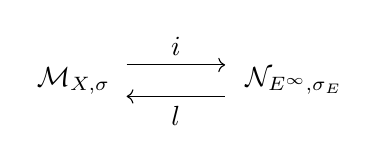
\begin{tikzpicture}
      \node (A) at (-1.3, 0)   {$\cM_{X, \sigma}$};
      \node (B) at (1.5, 0)    {$\cN_{E^\infty, \sigma_E}$};
      \node (C) at (-.75, .2)  {};
      \node (D) at (.75, -.2) {};
      \node (E) at (.75, .2)   {};
      \node (F) at (-.75,-.2)  {};
        
      \draw[->] (C) -- node[above] {$i$}      (E);
      \draw[<-] (F) -- node[below] {$l$} (D);
    \end{tikzpicture}$$ 
  \end{figure}
  is a natural bijection.
\end{prop}

Being so convinced that we can induce the new dynamical system on $E^\infty$ and recover information from it due to the bijection, we give several facts about the relationship between important properties of the original and induced system.

\begin{fact}
  The entropy of the induced measure is $h_{i(\mu)}(\sigma_E) = \frac{h_\mu(\sigma)}{\mu(E)}.$
\end{fact}

\begin{fact}
  Given some observable $\phi \in C(X, \RR)$, we can define an observable for $E^\infty$,
  $$\phi_E = \Sigma_{k=0}^{\tau_E(x)-1}\phi(\sigma^k(x))$$

  which gives a map from the integral with respect to the orginal measure to the integral with respect to the induced measure, 
  $$\int\phi d\mu \mapsto \int_E \left(\Sigma_{k=0}^{\tau_E(x)-1}\phi(\sigma^k(x))\right)d\mu = \frac{\int_E \phi d\mu}{\mu(E)} = \int\phi_E d\mu_E$$
  ???
\end{fact}
\begin{fact}
  The free energy of the induced measure is $F_{\mu_E, \sigma_E}(\phi_E) = \frac{F_{\mu, \sigma}(\phi)}{\mu(E)}.$
\end{fact}


\subsection{Entropy of Coded Shifts}\cite[L12]{wolf}
// TODO: wait for 05/03 lecture

\subsection{Examples of Computing Entropy of Shift Spaces}
// TODO: add examples from 04/26

\subsection{Questions}
\begin{enumerate}
  \item Is every shift a coded shift?
  \item I don't understand the paragraph about how to decompose a general measure into ergodic measures.
  \item definition of basin seems wrong.
  \item what's that about shift spaces having unique equilibrium state?
  \item defining the induced integral over an observable?
\end{enumerate}
\newpage




% ----------------------------------------------
\appendix
\section{Quick Reference Sheet}
{\setlength{\parindent}{0pt} 
\begin{multicols}{2}

% ----------------------
\subsection{Shift Spaces}
\begin{itemize}[leftmargin=2.3em]
\item[def:] TODO  
\end{itemize}

\textbf{SFTs}  
\begin{itemize}[leftmargin=2.3em]
\item[idea:] described by a transition matrix (adjacency matrix or graph with 1-1 labeling)  
\item[idea:] defined by a language OR a forbidden word set  
\item[def:]   
\item[thm:] every SFT is topologically conjugate to a 1-step SFT (1-step on the bottom of the commutative square by the higher block representation w/ mad forbidden word len 2)  
\item[e.g.] Full shift   
\item[e.g.] Golden mean shift  
\end{itemize}

\textbf{Sofic shifts}
\begin{itemize}[leftmargin=2.3em]
  \item[idea:] described by a finite labeled directed graph over a finite alphabet
  \item[def:]  
  \item[e.g.] Even shift TODO
  \item[thm:] Sofic Shifts are always factors of some SFT. (Sofic on the bottom of the commutative square).
\end{itemize}

\textbf{Coded shifts}
\begin{itemize}[leftmargin=2.3em]
  \item[idea:] described by an irreducible countable directed labeled graph over a finite alphabet.
  \item[idea:] described by countable generating set 
  \item[def:] Let $\cG$ be a TODO: define unique representation
  \item[e.g.] S-gap shifts TODO
  \item[e.g.] Beta shifts TODO
  \item[thm:] the class of coded shifts contains both sofic shifts and SFTs.
\end{itemize}

\textbf{Topological entropy of shifts}
\begin{itemize}[leftmargin=2.3em]
  \item[idea:] count distinguishable orbits under some margin of measurement like pixels on a screen, 
  \item[idea:] how surprised are you by the next letter? what is the information exponential growth rate as words get longer
  \item[def:] (general) exponential growth of the maximal $n-\epsilon$ separated set
  \item[def:] (shifts) Let $X \in \Sigma_{\inf}$ be a shift space. Then $h_{top}(X) = \lim_{n \rightarrow \infty} \frac{1}{n} \log |\cL_n(X)|$.
  \item[thm:] the entropy of an SFT described by an irreducible transition matrix $A$ is $\log \lambda$ where $\lambda$ is the Perron eigenvalue of $A$.
  \item[thm:] the entropy of an SFT described by a matrix which is the product of irreducible transition matrices $A_i$ is $\log \lambda_i$ where $\lambda_i$ is the max of the perron eigenvalues of the $A_i$.
\end{itemize}


% -------------------------
\subsection{Ergodic Theory}  
\begin{itemize}[leftmargin=*]
  \item[-] 
\end{itemize}

\textbf{Measure theory basics}
\begin{itemize}[leftmargin=2.3em]
  \item[def:] let $X$ a topological space, $\Sigma \subseteq P(X)$ is a \underline{sigma algebra} if 1) $X, \phi \in \Sigma$, 2) arbitrary unions are in $\Sigma$, 3) complements are in $\Sigma$. (2 and 3 $\Rightarrow$ arbitrary intersections)
  \item[def:] dthe \underline{Borel sigma algebra} is $\cB$ the smallest sigma algebra which contains all open sets according to the provided topology. 
  \item[def:] a \underline{measure} is a function $\mu: \cB \rightarrow \RR_+$ such that 1) for a pairwise disjoint set of $A_i \in \cB$, $\mu(\cup A_i) = \sum \mu (A_i)$. TODO what else 
  \item[def:] \underline{$\cM_{X,T}$} for $(X,d)$ compact metric space, $T: X \rightarrow X$, it is the set of all invariant Borel probability measures on $X$, i.e. $\mu(A) = \mu(T^{-1}(A))$
  \item[thm:] $\cM_X$ has the weak-* topology: the smallest topology where $\mu \rightarrow \int \phi d\mu$ is continuous for all $\phi \in C(X, \RR)$. (i.e. $\mu_n \rightarrow \mu$ iff. $\int \phi d\mu_n \rightarrow \int \phi d\mu$)
  \item[thm:] $\cM_X$ is compact and non-empty in the weak-* topology. 
  \item[thm:] the weak-* topology is metrizable by the Wasserstein-Kantorovich metric between probability distributions. 
\end{itemize}

\textbf{Relevant Ergodic Theory}
\begin{itemize}[leftmargin=2.3em]
\item[def:] a set is \underline{convex} if drawing a line between any two points stays within the set. For $\cM_X$,  $\mu_1, \mu_2 \in \cM_X \Rightarrow \alpha\mu_1 + (1-\alpha)\mu_2 \in \cM_X$ for $\alpha \in [0,1]$.
\item[def:] $\mu \in M_X$ is \underline{ergodic} if $\mu(A) = 1$ or $\mu(A) = 0$ for all $T$-invariant subsets $A$.
\item[thm:] $\cM_E$ the extreme points of $\cM_X$ are precisely the ergodic measures.
\item[def:] the \underline{basin} of a measure is the set $\cB(\mu) = \{x \in X : \lim_{n \rightarrow \infty} \sum_{k=0}^{n-1}\delta_{f^{k}(x)} = \mu\}$ (TODO: how is this related to the time average?)
\item[def:] \underline{measure of maximal entropy} is a $\mu$ s.t. $h_\mu(f) = h_{top}(f)$.
\end{itemize}

% -----------------------
\subsection{Computability}

\end{multicols}
}



\newpage
\section{Lecture index}  

\begin{tabular}{|c|c|}\hline
  L1 & 01/25 \\ \hline
  L2 & 02/01 \\ \hline
  L3 & 02/15 \\ \hline
  L4 & 02/22 \\ \hline
  L5 & 03/02 \\ \hline
  L6 & 03/08 \\ \hline
  L7 & 03/15 \\ \hline
  L8 & 03/22 \\ \hline
  L9 & 04/05 \\ \hline
  L10 & 04/19 \\ \hline
  L11 & 04/26 \\ \hline
  L12 & 05/03 \\ \hline
\end{tabular}

\printbibliography

\end{document}
